\chapter{Software Backbone:}
Embedded systems of this sort use software; ubiquitous information right ? But apparently, "software" is a universe that allows for countless philosophies and approaches. 

For our platforms, we want software to be modular, you can pick software and use elsewhere, this notion already exists, it's libraries, packages, modules...etc But how do we make it as versatile as our systems are aiming to get ? One possible way to do this is by dividing software into layers, for now, 3 layers suffice; 
-The Logic-Software layer (Functional/OOP); takes care of behaviours and logic 
-The Software-Middlewear layer (RTOS)
-The Hardware layer (HAL);

one way to do this is by using a hexagonal architecture %refer to this here

\begin{figure}
    \centering
    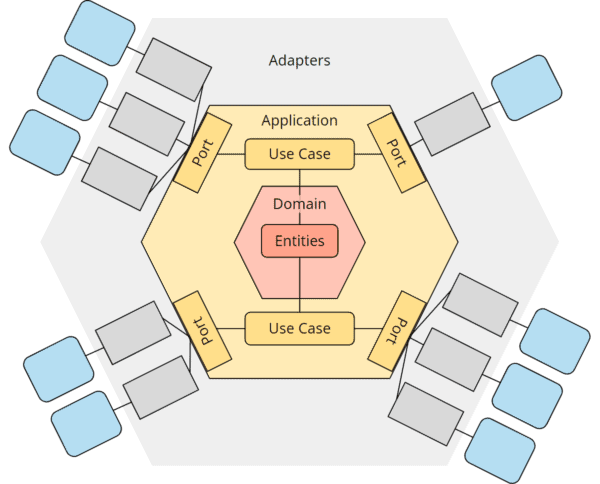
\includegraphics[width=0.5\linewidth]{image.png}
    \caption{Enter Caption}
    \label{fig:placeholder}
\end{figure}

\section{Introduction}

Designing reliable software for cyber-physical systems (e.g.\ drones, robots, autonomous vehicles) requires more than just writing code that runs. 
It requires a principled approach to structuring the software such that logic, hardware interaction, and operating system details are separated. 
This separation fosters modularity, portability, and long-term maintainability. 
In this chapter we outline a general philosophy for embedded systems architecture using a layered approach inspired by ports-and-adapters (also known as the hexagonal architecture).

\section{Motivation}

Embedded systems integrate three worlds:
\begin{enumerate}
    \item \textbf{The application logic} --- the mathematical and algorithmic core, e.g.\ control laws, estimators, and data fusion.
    \item \textbf{The hardware interface} --- the code that speaks to sensors, actuators, communication buses, and storage devices.
    \item \textbf{The middleware} --- the operating system or runtime services that schedule tasks, manage concurrency, and orchestrate communication.
\end{enumerate}

Without clear boundaries, these three concerns tend to intertwine. 
The result is fragile software that is difficult to port to new hardware or to test in isolation. 
A layered philosophy addresses this by enforcing strict separation of responsibilities.

\section{Core Logic Layer}

At the center lies the \emph{core logic layer}. 
This layer contains:
\begin{itemize}
    \item State estimation and sensor fusion algorithms.
    \item Controllers (e.g.\ PID, cascaded angle-rate loops).
    \item Mixers that translate control outputs into actuator commands.
    \item Safety mechanisms such as failsafe behaviour.
    \item Telemetry formatting and semantics.
\end{itemize}

A key design rule is that the core layer must remain \textbf{platform independent}. 
It does not include device drivers, operating system calls, or hardware registers. 
Instead, it depends only on abstract interfaces that define what the system \emph{requires} (e.g.\ ``read IMU sample'', ``write motor outputs'', ``send telemetry'').

\section{Ports and Adapters}

Between the core and the physical world sit the \emph{ports and adapters}. 
\begin{itemize}
    \item \textbf{Ports} are abstract interfaces, defined in the core, that describe required capabilities such as reading a sensor, commanding an actuator, or storing configuration data.
    \item \textbf{Adapters} are concrete implementations of these ports for a specific platform. 
          For example, one adapter may implement the motor control port using PWM timers on an ARM microcontroller, while another implements the same port using LEDC on an ESP32. 
\end{itemize}

This inversion of dependencies (the core depends only on abstractions, not concrete drivers) allows us to swap hardware, libraries, or protocols without touching the control logic.

\section{Middleware Layer}

The middleware layer encompasses the runtime environment and operating system services:
\begin{itemize}
    \item Task scheduling and priorities (e.g.\ FreeRTOS tasks at fixed update rates).
    \item Communication orchestration (e.g.\ network discovery, pairing protocols).
    \item Synchronization primitives for safe access to shared state.
\end{itemize}

The middleware injects concrete adapters into the core at startup. 
It is the \emph{composition root}, responsible for wiring together the system: instantiating drivers, providing clock sources, and starting scheduled tasks.

\section{External Entities}

Finally, beyond the software layers are the \emph{external entities}:
\begin{itemize}
    \item Physical hardware such as sensors, actuators, and microcontrollers.
    \item Human operators and controllers.
    \item Ground stations or monitoring clients.
\end{itemize}

These interact with the system exclusively through the defined adapters and ports. 
This ensures that the boundary between ``inside the software'' and ``outside in the world'' is explicit and testable.

\section{Benefits of the Layered Philosophy}

This separation yields several advantages:
\begin{enumerate}
    \item \textbf{Portability}: Core logic runs unchanged on different microcontrollers or operating systems, as long as suitable adapters exist.
    \item \textbf{Testability}: The core can be simulated on a desktop computer with mock adapters, enabling unit tests and hardware-in-the-loop simulation.
    \item \textbf{Maintainability}: Hardware upgrades or protocol changes only require replacing or extending adapters, not rewriting algorithms.
    \item \textbf{Clarity}: A well-defined architecture provides a conceptual map, reducing coupling and making reasoning about safety and performance easier.
\end{enumerate}

\section{Conclusion}

The general philosophy presented here is applicable to a wide range of embedded and control systems. 
By clearly distinguishing between the logic, the hardware interface, and the middleware, engineers can create software that is modular, reusable, and robust. 
This layered approach transforms complex projects from monolithic and brittle implementations into structured systems that can evolve over time without losing reliability.
